\documentclass[fontset=windows]{article}
\usepackage[margin=1in]{geometry}%设置边距,符合Word设定
\usepackage{ctex}
\usepackage{setspace}
\usepackage{lipsum}
\usepackage{graphicx}%插入图片
\usepackage{subcaption}
\graphicspath{{Figures/}}%文章所用图片在当前目录下的 Figures目录

\usepackage{hyperref} % 对目录生成链接,注:该宏包可能与其他宏包冲突,故放在所有引用的宏包之后
\usepackage{amsmath}
\usepackage{mathtools}
\usepackage{marginnote}
\usepackage{tcolorbox}
\usepackage{enumitem}

\hypersetup{colorlinks = true,  % 将链接文字带颜色
	bookmarksopen = true, % 展开书签
	bookmarksnumbered = true, % 书签带章节编号
	pdftitle = 基于图像的三维重建学习笔记, % 标题
	pdfauthor =Gukazma} % 作者
\bibliographystyle{plain}% 参考文献引用格式

\renewcommand{\contentsname}{\centerline{Contents}} %经过设置word格式后,将目录标题居中


\title{\heiti\zihao{2} 基于图像的三维重建学习笔记}
\author{\songti Gukazma}
\date{\today}


\begin{document}
	\maketitle
	\thispagestyle{empty}

\begin{abstract}
	基于图像的三维重建学习笔记,附个人学习批注,并详细推导计算过程。
\end{abstract}

\tableofcontents

\section{特征提取及匹配}
\subsection{特征提取}
\subsubsection{Harris角点检测}

\begin{flalign*}
&& E(u, v) &= \sum_{(x,y)}^{} w(x,y)[I(x+u,y+v)-I(x,y)]^2 &&  \\
\text{对}I(x+u,y+v)\text{一阶泰勒展开} && &\approx \sum_{(x,y)}^{} w(x,y)[I(x,y)+\frac{\partial I}{\partial x}(x,y)u +\frac{\partial I}{\partial y}(x,y)v-I(x,y)]^2 &&\\
 && &= \begin{bmatrix}u \\v\end{bmatrix}^T \mathbf{H} \begin{bmatrix}u \\v\end{bmatrix} 
&&
\end{flalign*}
\begin{tcolorbox}
二元函数函数一阶泰勒展开推导:
\begin{flalign*}
f(x,y) &\approx f(x_0,y_0) + f_{x}'(x_0,y_0)(x-x_0)	+ f_{y}'(x_0,y_0)(y-y_0)\\
\text{令$x=x+u,y=y+v$:}\\ 
f(x+u,y+v) &\approx f(x_0,y_0) + f_{x}'(x_0,y_0)(x+u-x_0)+f_{y}'(x_0,y_0)(y+v-y_0)\\
\text{令$x_0=x,y_0=y$:}\\ 
&= f(x,y) + f_{x}'(x,y)(x+u-x)+f_{y}'(x,y)(y+v-y)\\
&= f(x,y) + f_{x}'(x,y)u+f_{y}'(x,y)v
\end{flalign*}
\end{tcolorbox}

其中$\mathbf{H}$为Harris矩阵:
\begin{equation*}
H=
\begin{bmatrix}
	\sum_{(x,y)}^{}w(x,y)(\frac{\partial I}{\partial x}(x,y))^2 & \sum_{(x,y)}^{}w(x,y)(\frac{\partial I}{\partial x}(x,y)\frac{\partial I}{\partial y}(x,y)) \\
	\sum_{(x,y)}^{}w(x,y)(\frac{\partial I}{\partial y}(x,y)\frac{\partial I}{\partial y}(x,y)) & \sum_{(x,y)}^{}w(x,y)(\frac{\partial I}{\partial y}(x,y))^2
\end{bmatrix}
\end{equation*}

\begin{figure}[h]
    \centering
    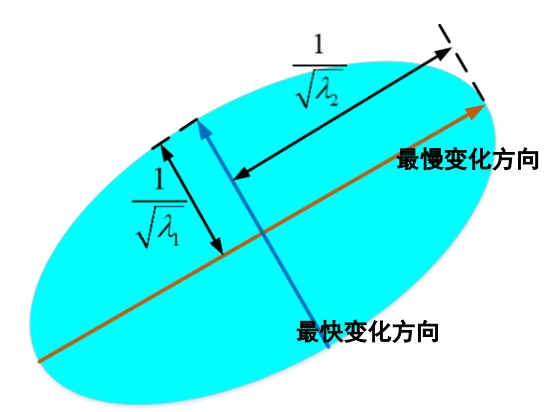
\includegraphics[height=2in]{harrisShape.png}
    \caption{Harris矩阵特征椭圆形}
    \label{fig:harrisShape}
\end{figure}

Harris 矩阵H的特征值分析:
\begin{equation*}
	SVD(H) = U \sum V, (\lambda_1, \lambda_2), \lambda_1 > \lambda_2
\end{equation*}
\begin{itemize}[leftmargin=2cm]
	\item $\lambda_1 \approx \lambda_2$ 兴趣点位于光滑区域;
	\item $\lambda_1 > 0  \lambda_2 \approx 0$ 兴趣点位于边缘区域;$\lambda_1 > 0  \lambda_2 \approx 0$ 兴趣点位于边缘区域;
	\item $\lambda_1, \lambda_2 > 0$ 兴趣点位于角点区域。
\end{itemize}

Harris角点准则:
\begin{equation*}
	C = det(H) - ktrac(H)^2 = \lambda_1\lambda_2 - k(\lambda_1 + \lambda_2)^2, k = 0.04
\end{equation*}
\begin{itemize}[leftmargin=2cm]
	\item k的值越小, 检测子越敏感
	\item 只有当$\lambda_1$和$\lambda_2$同时取得最大值时,C才能取得最大值
	\item 避免了特征值分解,提高检测效率
\end{itemize}
这里使用非极大值抑制(Non-maximal Suppression)
选取局部响应最大值,避免重复的检测。
\subsubsection{LoG算子}
高斯算子取图像的周围几个像素取平均值,这样就能实现模糊图像,去除噪声的作用。
保留了图片的大致特征,就像人眯起眼睛看东西或者从不同距离看东西一样。

$\sigma$表示高斯核的大小,$\sigma$越大,则经过高斯卷积的图像越模糊。不同$\sigma$处理的图像就形成了一个三维的\textbf{尺度空间}。

\begin{figure}[h]
    \centering
    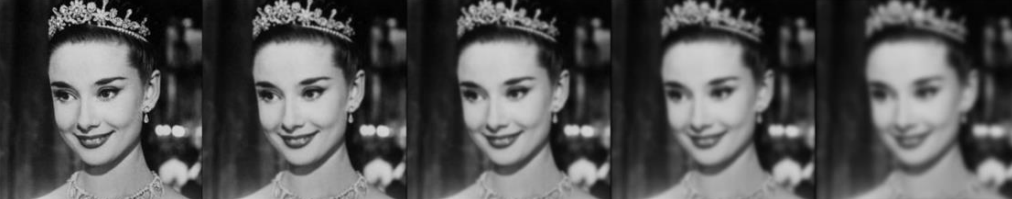
\includegraphics[height=1in]{LoG.png}
    \caption{尺度空间}
    \label{fig:harrisShape}
\end{figure}

对不同尺度下的图像求二阶导数,并取极值点,就得到了LoG算子:
\begin{equation*}
    \nabla^2L(x, y, \sigma_D)=(\frac{\partial^2L(x,y,\sigma_D)}{\partial x^2} + \frac{\partial^2L(x,y,\sigma_D)}{\partial y^2})*I(x,y)
\end{equation*}

尺度归一化LoG算子:

\begin{equation*}
    \nabla_{norm}^{2}L(x, y, \sigma_D)=\sigma_{D}^{2}(\frac{\partial^2L(x,y,\sigma_D)}{\partial x^2} + \frac{\partial^2L(x,y,\sigma_D)}{\partial y^2})*I(x,y)
\end{equation*}

不同尺度下的LoG响应值不具有可比性

\begin{figure}[h]
    \centering
    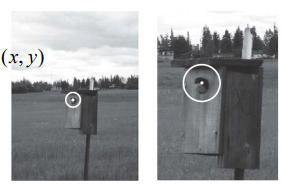
\includegraphics[height=1in]{不同尺度LoG极值点.png}
    \caption{不同尺度LoG极值点}
    \label{fig:harrisShape}
\end{figure}

需要计算位置空间和尺度空间寻找归一化LoG极值,作为特征点。

LoG特征检测结果效果好,但是计算量很大。(每个像素)
\begin{figure}[h]
    \centering
    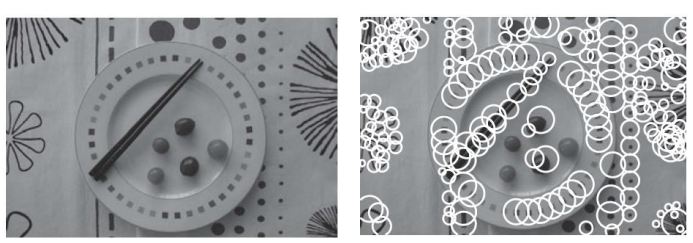
\includegraphics[height=2in]{LoG效果.png}
    \caption{LoG效果}
    \label{fig:harrisShape}
\end{figure}
\subsubsection{基于DoG算子的特征检测子(SIFT)}

\textbf{Lowe(2004)提出LoG近似等价于相邻尺度的高斯差分(DoG)}

高斯空间
\begin{equation*}
    L(x,y,\sigma) = G(x,y,\sigma) * I(x,y)
\end{equation*}

高斯差分(DoG)

\begin{flalign*}
    D(x,y,\sigma) &= (G(x,y,k\sigma) - G(x, y, \sigma)) * I(x,y)\\
    &= L(x,y,k\sigma) - L(x, y, \sigma)
\end{flalign*}

\textbf{DoG差分空间:} 

每个Octave的图像进行一次2倍的将采用,将采用得到的尺度$\sigma$为原来的两倍。

\begin{figure}[h]
\centering
\begin{minipage}[t]{0.48\textwidth}
\centering
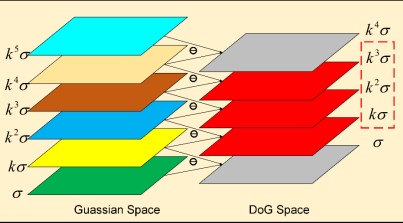
\includegraphics[width=6cm]{DoG差分Octave1.png}
\caption{Octave 1}
\end{minipage}
\begin{minipage}[t]{0.48\textwidth}
\centering
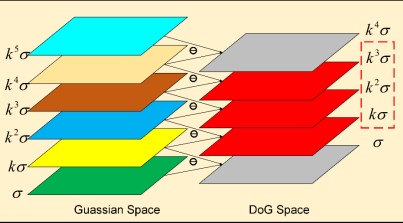
\includegraphics[width=6cm]{DoG差分Octave1.png}
\caption{Octave 2}
\end{minipage}
\begin{minipage}[t]{0.48\textwidth}
\centering
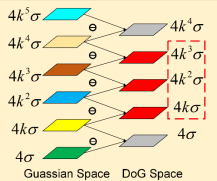
\includegraphics[width=6cm]{DoG差分Octave3.png}
\caption{Octave 3}
\end{minipage}
\end{figure}

阶数:$O = 3$

每阶的有效差分数:$S=3$  (有效差分数为去掉首尾的,图中DoG空间的红色部分)

每阶层数:$N=S+3$

这样设计的目的是保证每阶的DoG空间有效差分层最后一个的尺度正好等于下一阶的第一层尺度的一半。
这就使得DoG空间尺度上是连续、等间隔的。

\textbf{查找DoG空间离散极值点:} 

\begin{figure}[h]
    \centering
    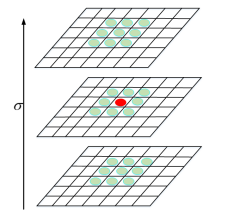
\includegraphics{DoG寻找极值点.png}
    \caption{DoG寻找极值点}
\end{figure}

在寻找极值点时,会比较上下两个尺度的图片中的除了自身以外的相邻的$4*4*3-1=47$个像素值。
当前像素值大于这相邻的其它47个像素值,则该点为极值点。

\textbf{通过泰勒展开近似查找亚像素DoG空间离散极值点:} 

利用二阶泰勒近似寻找极值点

\begin{flalign*}
\text{对$f(x_0)$进行泰勒二阶展开近似}\\ 
f(x) &\approx f(x_0) + \nabla f(x_0)^T(x-x_0) + \frac{1}{2}(x-x_0)^T\nabla^2f(x_0)(x-x_0) \\
\text{剔除常数项$f(x_0)$,并令$\delta x=x-x_0$得:}\\ 
f(\delta x) &= \nabla f(x_0)^T\delta x + \frac{1}{2}\delta x^T\nabla^2f(x_0)\delta x \\
\text{求一阶导,并令其为0:}\\ 
\frac{\partial f(\delta x)}{\partial \delta x} &= \nabla f^T(x_0) + \nabla^2f(x_0)\delta x = 0 \\
\text{整理上式得:}\\ 
\delta x &= -\nabla^2 f(x_0)^{-1} \nabla f^T(x_0)
\end{flalign*}

其中$\delta x$为在$x_0$点的近似极值点。

去除边缘点:

由于DoG在边缘处值较大,所以需要尽量避免检测到图像边缘点。

\begin{equation*}
    \frac{trace(\boldsymbol{H})}{Det(\boldsymbol{H})} < \frac{(r+1)^2}{r}, r=10
\end{equation*}

计算主方向:

\begin{figure}[h]
    \centering
    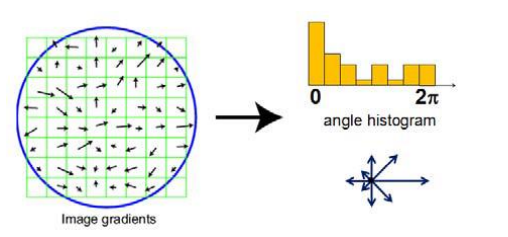
\includegraphics{SIFT主方向.png}
    \caption{SIFT主方向}
\end{figure}

计算一个锚点周围$8x8$个像素的8个方向的梯度,并取每个像素的最大梯度值的方向作为该像素的方向,
计算得到角度直方图,取最大值作为主方向。

\begin{figure}[h]
    \centering
    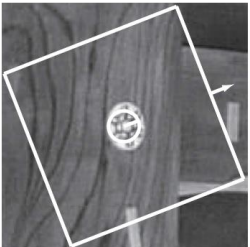
\includegraphics{SIFT主方向旋转.png}
    \caption{SIFT主方向旋转}
\end{figure}

为了使得特征点具有旋转不变性,需要图像向主方向旋转。


为了使得特征具有亮度不变性,故需要对每个像素减去均值并除以方差

\begin{equation*}
    I^* = \frac{I-u}{\sigma}
\end{equation*}


特征描述符:

统计局部梯度信息,将区域划分成4x4的block,每个block内统计梯度方向的直方图(高斯加权梯度
作为系数)

\begin{figure}[h]
    \centering
    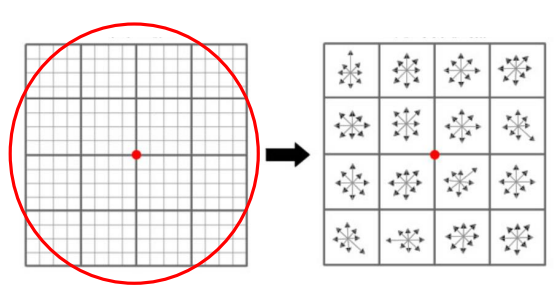
\includegraphics{特征描述符.png}
    \caption{特征描述符}
\end{figure}


\begin{figure}[h]
    \centering
    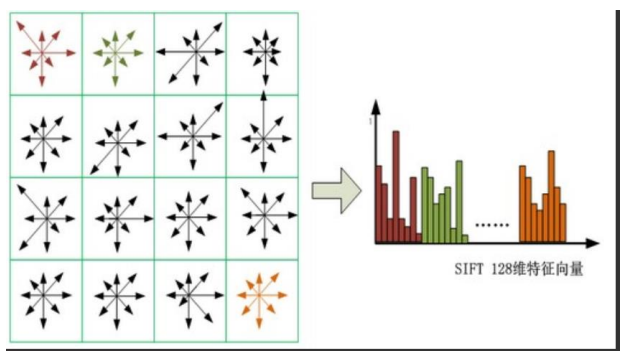
\includegraphics{特征描述符直方图.png}
    \caption{特征描述符直方图}
\end{figure}

\bibliography{books}
\end{document}